\section{Diskussion}
\label{sec:Diskussion}
Mit einem Studentschen t-Testes soll die Übereinstimmung der Größe $\frac{1}{\lambda}$
überprüft werden. Diese wurde auf drei verschiedenen Wegen bestimmt: Durch die direkte 
Wellenlängenmessung, durch die direkte Frequenzmessung und durch die Schwebungsmethode.

\begin{table}
	\centering
	\caption{Messergebnisse der Größe $\frac{1}{\lambda}$.}
	\label{tab:alam}
	\begin{tabular}{ccc}
		\toprule
		Methode & $\frac{1}{\lambda}$ / $\frac{1}{\si{\meter}}$ & Anzahl der Einzelmessungen \\
		\midrule
		Wellenlänge & $\num{59.5(2)} \, \si{\meter}$ & 5         \\
		Frequenz & $\num{59.76(25)} \, \si{\meter}$ & 20  \\
		Schwebung & $\num{60.74(30)} \, \si{\meter}$ & 20  \\
		\bottomrule
	\end{tabular}
\end{table}
Der Studentsche t-Test ermöglicht es die Kongruenz der Messergebnisse (aufgetragen in Tabelle
\ref{tab:alam}) zu diskutieren.

Der zu bestimmende Wert \cite{ttest} für die  Wahrscheinlichkeit eines systematischen Fehlers 
ergibt sich zu
\begin{equation}
	\label{eqn:amina}
	t = \frac{x_1 - x_2}{\sqrt{\frac{1}{m} + \frac{1}{n}} S} \, \mathrm{,}
\end{equation}
mit 
\begin{equation}
	\label{eqn:koyim}
	S^2 = \frac{(m-1)s_1^2 + (n-1)s_2^2}{m+n-2} \mathrm{.}
\end{equation}
Die Größen $x_1$ und $x_2$ entsprechen den Mittelwerten aus den entsprechenden Messreihen, 
$s_1$ und $s_2$ sind die Fehler der Mittelwerte und die Größen $m$ und $n$ stellen die 
Anzahl der Einzelmessungen jeder Messreihe dar, wobei $m+n-2$ der Anzahl der Freiheitsgrade
entspricht.
Aus den Formeln \eqref{eqn:amina} bzw. \eqref{eqn:koyim} und den Werten aus Tabelle 
\ref{tab:alam} lassen sich die drei verschiedenen Methoden zur Bestimmung der Größe 
$\frac{1}{\lambda}$ miteinander vergleichen.

Der Vergleich der Bestimmung der Wellenlängenmessung und der direkten Frequenzmessung liefert 
den Wert 
\begin{equation*}
	t_{\mathrm{wf}} = 2,148
\end{equation*}
und damit die Wahrscheinlichkeit für einen systematischen Fehler von $95\%$ \cite{tttest}.

Für den Vergleich von der Wellenlängenmessung und der Schwebungsmethode ergibt sich
\begin{equation*}
	t_{\mathrm{ws}} = 8,698 \mathrm{.}
\end{equation*}
Daher kann nach dem Studentschen t-Test zu $100\%$ von einem systematischen Fehler ausgegangen 
werden wie bei dem Vergleich von der direkten Frequenzmessung und der Schwebungsmethode
mit 
\begin{equation*}
	t_{\mathrm{fs}} = 11,223 \mathrm{.}
\end{equation*}
Insgesamt lässt sich sich eine geringe Diskrepanz bei der Bestimmung der Größe $\frac{1}{\lambda}$ mit den drei verschiedenen Methoden feststellen.
\begin{figure}
	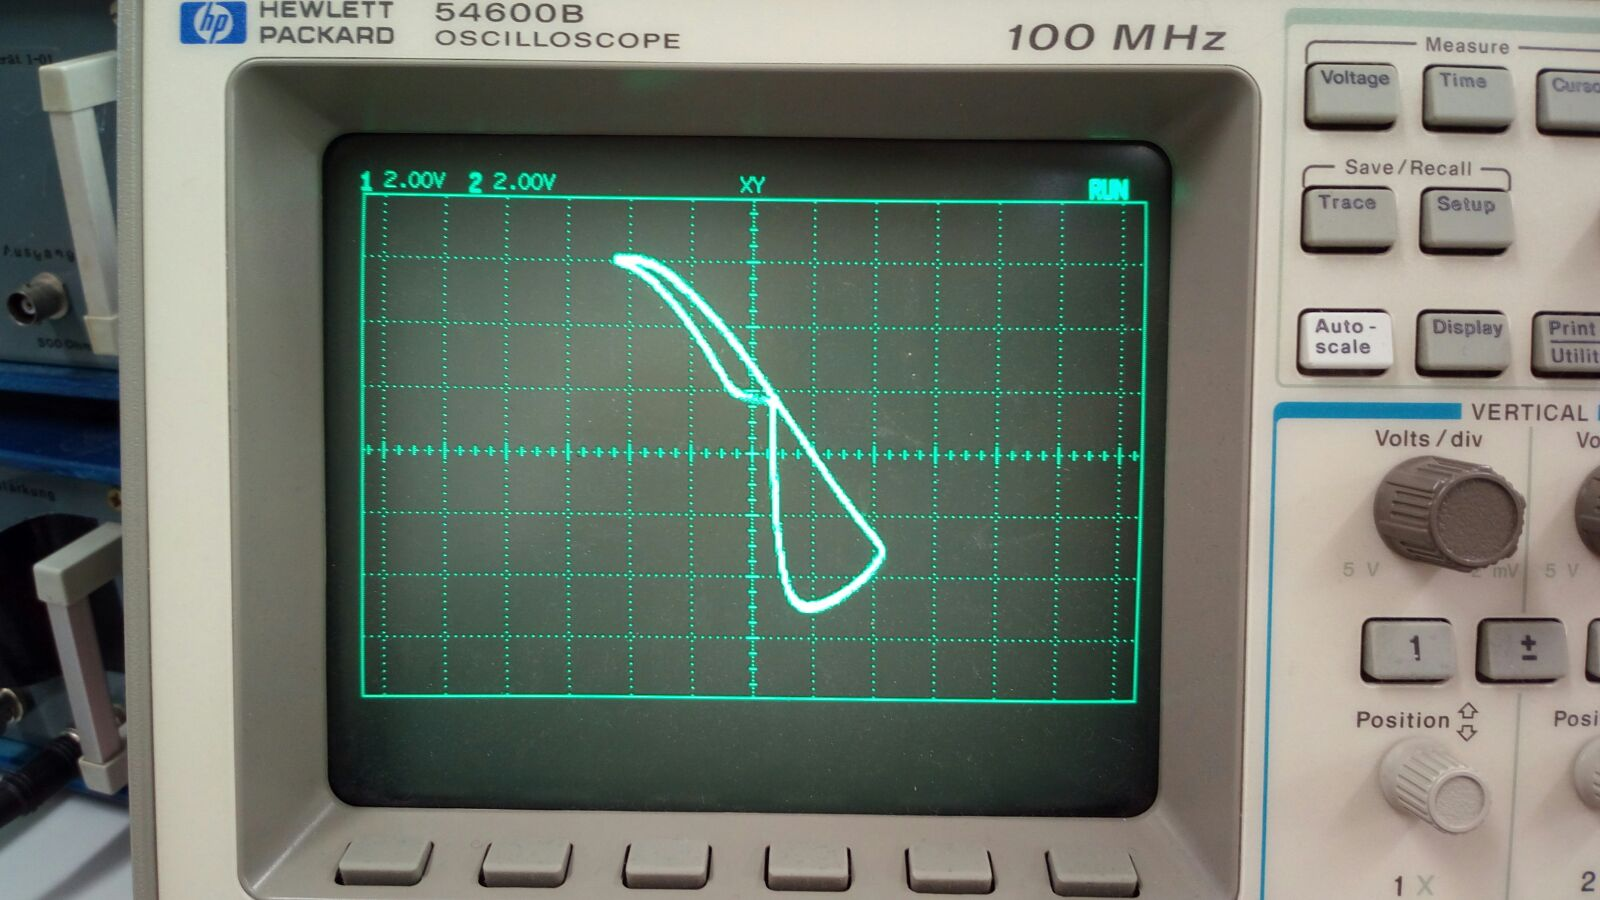
\includegraphics[width=0.9\textwidth]{Bilder/lissajou.jpeg}
	\caption{Bestmöglichste Entartung der LISSAJOUS-Figuren zu Geraden auf dem Oszilloskop.}
	\label{fig:Lisas}
\end{figure}
